
\chapter{Introduction}
\label{chap:intro}
"Which digital camera should I buy? Which movie should I rent? Which book should I buy for my next vacation?" These are some situations where people have to make decisions about how they are going to spend money, or in a broader level, about their future.
Traditionally, people have used a variety of strategies to solve such decision making problems: conversations with friends, obtaining information from a trusted third party, hiring an expert team or simply follow the crowd. It would be great to have an affordable personal advisor who helps us make good decisions efficiently.
The construction of systems that supports a user in his (online) decision-making is the main goal of the field of recommender systems. In particular, the goal of recommender systems is to provide easily accessible, high-quality recommendations for a large user community.
Recommender Systems are broadly classified into three categories: Collaborative, Content Based and Knowledge Based.

\section{Collaborative Recommender Systems}
 The main idea in these systems is that if users share the same interests in the past - if they viewed or bought the same books - they will also have similar tastes in the future. This technique is also called as \textit{Collaborative Filtering}. Pure CF based approaches do not require the additional knowledge about underlying users/items. Hence, the algorithms are usually domain independent. Most commercial recommender sytems use collaborative filtering for recommending items.
There are two approaches to do CF: Memory Based Approaches and Model Based Approaches

\subsection {Memory Based Approaches}
In this approach, the original rating matrix is held in memory and directly used to generate predicted ratings and recommendations. There are two popular memory based approaches:\\
\textbf{User based Nearest Neighbor(NN) Recommendation:} Given a user \textit{u}, the system computes top \textit{K} similar users to \textit{u} according to a pre-defined similarity measure. It recommends those items to user that haven't been rated/purchased by \textit{u} but liked by the top \textit{K} similar users.\\
\textbf{Item based NN Recommendation:} Given a user \textit{u}, the system recommends items that have received similar ratings to the ones that \textit{u} has previously liked.
 


\subsection {Model Based Approaches}
As opposed to memory based approaches that use the ratings matrix to directly generate predictions, model based approaches learn models corresponding to each item and each user from ratings matrix and the learned models are used to make predictions at run time.
Model based approaches perform well in practice for large datasets.
Matrix factorization is a popular model based approach. The superiority of matrix factorization techniques over traditional CF in improving prediciton accuracy was clearly seen during The Netflix prize competition.
Broadly speaking, matrix factorization methods derive a set of latent(hidden) factors from the rating patterns and characterize each item and user as vectors of these factors.
In the movie domain, such latent factors can correspond to some aspects of a movie like genre, but most of them are completely uninterpretable (\cite{koren})


\subsection{Limitations of CF}
\label{sec:limCF}
In real-world applications, the user-item ratings matrix tends to be very sparse, as customers generally provide ratings for very few items. CF systems have a limitation called the "cold-start problem". It has two aspects - how to recommend items who has given zero/very low number of ratings; and how to recommend those items that haven't received ratings yet.

%

%

\section{Content based recommender systems}
Content based recommender systems rely on item descriptions and user profiles to recommend items.
If the system knows that "Harry Potter" is a fantasy novel and the user \textit{Alice} has always like fantasy novels, the system can recommend the new "Harry Potter" book right away. So the system need not rely on the existence of a large user base to generate recommendations.
It overcomes the cold-start problem described in the section ~\ref{sec:limCF}. However, item characteristics are hard to acquire normally and hence, they have to be entered manually into the system, which can be potentially expensive for some domains.

\section{Knowledge based recommender systems}
Typically, we do not buy a house, a car or a computer very frequently. In such a scenario, a pure CF system will not perform well because of the low number of available ratings
In more complex and high-risk product domains such as cars, customers often want to define their requirements explicitly - for example, "the maximum price of the car is $x$ and the color should be \textit{black}". In knowledge based systems, recommendations are made taking into account the explicit user preferences and the rich knowledge base available.

Recommendation process of knowledge-based recommender applications is highly interactive, a foundational property that is a reason for their characterization as \textit{\textbf{conversational systems}}. The recommender system that we consider in this project is a conversational system.\\
Conversational systems assume that a user's initial query is merely a starting point for search, perhaps even an unreliable starting point. The job of the recommender system is to help the user refine his initial preference query as the interactions proceed.

\subsection{Critiquing}

\begin{figure}
\centering
\begin{minipage}{.5\textwidth}
  \centering
  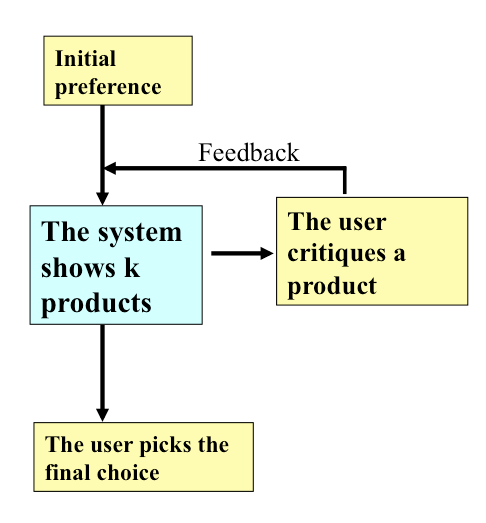
\includegraphics[width=1\linewidth]{figures-bharath/critiquing.png}
  \captionof{figure}{Critiquing}
  \label{fig:test1}
\end{minipage}%
\begin{minipage}{.5\textwidth}
  \centering
  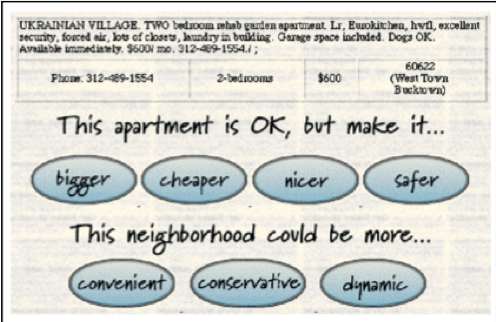
\includegraphics[width=1\linewidth]{figures-bharath/rentMe.png}
  \captionof{figure}{RentMe Recommender System: \cite{burkeRentMe}}
  \label{fig:rentMe}
\end{minipage}
\end{figure}
\textit{\textbf{Critiquing}} is one of the most popular forms of feedback in conversational recommender systems. In each interaction cycle, the user is presented with a list of products.
User selects a product and expresses directional preference(s) over one or more item feature values. For example, one might indicate that he/she is looking for a less expensive restaurant or a more formal setting. These are two individual critiques, first critique being on the \textit{price} attribute and the second critique on the \textit{setting} attribute. The recommender updates it's user model according to this feedback provides another set of products and proceeds to the next recommendation cycle. This continues till the user finally chooses a product.

\textit{\textbf{Unit critiques}} allow users to express their preference over one attribute in each interaction cycle. \textit{\textbf{Compound critiques}} enable users to input their preferences on several attributes at a time. This can potentially shorten the number of interaction cycles in finding a target product.
The early FindMe Systems \cite{burkeEarlierSystems} had \textit{static} critiques. The critiques wouldn't change when users selected a particular critique. 
This can lead to some serious limitations.
For example, the critique 'cheaper' would continue to be visible, even if there are no cheaper apartments available and when user clicks on 'cheaper', there would be no results displayed at all.
Static critiques also do not represent the best set of tweaks that a user will want to make given his preference model.
The notion of \textit{dynamic critiquing} was first proposed by \cite{mccarthy2004dynamic} to overcome the limitations of static critiques.
Compound critiques are generated on-the-fly for each recommendation cycle. Dynamic critiquing has been shown to improve user-experience and lower the average number of interaction cycles it takes for a customer to find his desired product


\section{Our contribution: Improvements to MAUT based recommendation}
\section{Organization of the Thesis}

